\documentclass[]{IEEEtran}

% Your packages go here
\usepackage[utf8]{inputenc}
\usepackage{graphicx}
\usepackage{float}
\usepackage{listings}
\usepackage{xcolor}
\usepackage{amsmath}
\usepackage{hyperref}
\usepackage{url}
%listings settings
\definecolor{codegreen}{rgb}{0,0.6,0}
\definecolor{codegray}{rgb}{0.5,0.5,0.5}
\definecolor{codepurple}{rgb}{0.58,0,0.82}
\definecolor{backcolour}{rgb}{0.95,0.95,0.92}
\definecolor{codeblue}{rgb}{0,0.8,0.99}
\definecolor{codeyellow}{rgb}{0.6,0.5,0}


\lstdefinestyle{vim_like}{
  backgroundcolor=\color{backcolour},   
  commentstyle=\color{codegreen},
  keywordstyle=\color{codeyellow},
  numberstyle=\tiny\color{codegray},
  stringstyle=\color{codepurple},
  basicstyle=\ttfamily\footnotesize,
  breakatwhitespace=false,         
  breaklines=true,                 
  captionpos=b,                    
  keepspaces=true,                 
  numbers=left,                    
  numbersep=5pt,                  
  showspaces=false,                
  showstringspaces=false,
  showtabs=false,                  
  tabsize=2
}
\lstset{style=vim_like}

\newcommand\todolist[1]{\textcolor{red}{#1}}

\markboth{MC949/MO446 Computer Vision}{}

\begin{document}
  \title{Project 2 - Augmented Reality}
  \author{Iury Cleveston (RA 230216), Leonardo Rezende (RA 262953) and Thales Oliveira (RA 148051)
    \thanks{ra230216@students.ic.unicamp.br, ra262953@students.ic.unicamp.br, ra148051@students.ic.unicamp.br}
  }
  \maketitle
  
  \begin{abstract}
    In this project, we were given the task of performing Augmented Reality (AR) task in media, in this case, a video. The goal was to make an image appear in every single frame of the video, in this case, a specific target on the video is always substituted by the image, while the camera changes position, orientation and focal distance. In order to fulfill the requirements, the algorithm implemented deals with image descriptors for every frame pair to find the target, a matching algorithm to hypothesize matches and a RANSAC with least squares methodology to calculate the transform between frames. We were able to generate AR video, and the limitations of our implementation are explained in this report.
  \end{abstract}
  
\section{Introduction}
This work, developed by Group 8 of Computer Vision Course (2nd Semester/2019), has the goal of generating Augmented Reality videos, using a simple approach. In this sense, it is desired to substitute, in every single frame of the video, a specific region, which is called in this work "target", by another image, considering that the camera is moving freely in the environment (changing horizontal/vertical positions, rotating (counter)clockwise, zooming-in/out). To do such tasks, a pipeline was implemented and every single task divided. An image descriptor algorithm was implemented, to be able to locate the target frame within a video frame. For matching the target frame between 2 consecutive frames, a matching algorithm was implemented, to map candidate keypoints between those frames. Using those candidate matches, an algorithm using RANSAC and Least Squares was implemented to find the affine transform between frames. Therefore, we generate an AR video based on the original video, the descriptor, the matching algorithm and the affine transform algorithm. The following sections explain the implemented work, and the tests applied to the code.  

\section{Implemented Algorithm}
In this section, it is presented the implemented algorithm in this project. The code is distributed into five principal Python files, named \textbf{affine\_transform.py}, \textbf{ar.py}, \textbf{main.py}, \textbf{matching.py} and \textbf{sift.py}. The \textbf{affine\_transform.py} file contains the \textit{AffineTransform} class, which implements the RANSAC with Least Squares to calculate best Affine transform for the candidate matches. The \textbf{ar.py} file contains the \textit{AR} class, which implements the video manipulation, calls for the descriptor, matching and affine transform functions and pasting image into the target. The \textbf{main.py} file does the calls to the \textit{AR} class. The \textbf{matching.py} contains the \textit{Matching} class, which calculates possible candidate matches from the keypoints and its descriptions calculated by the implementation done in the \textbf{sift.py} file. The following subsections explains main implementation decisions done in key parts of the project, based on pipeline execution order.


\subsection{Implementation of the Pipeline}

The pipeline for processing the video was implemented in the AR() class and consists of the following steps:

\begin{itemize}
  \item loading the video and processing it frame-by-frame;
  \item loading target and source images;
  \item detection and description of keypoints for each frame using SIFT;
  \item matching the keypoints for each frame pair using the k-nearest neighbors algorithm;
  \item affine matrix calculation using the least squares and RANSAC algorithms;
  \item applying the transformations to the source image in each frame;
  \item separation of the target image from the frame and replace with the transformed source image. 
\end{itemize}


\subsection{Interest Points and Descriptors}

 The SIFT feature detection algorithm was chosen to extract the descriptors from each frame of the video. The reason for SIFT is that it's robust and can detect features invariant to translation, rotation and scale. It compares different image sizes to look for \textit{keypoints}. For this, a pyramid of Gaussian is generated (and an example can be seen at Fig. \ref{fig:gp}) and then the difference between the pyramid layers is calculated to generate a new octave with lesser information to look at. This new octave is called Difference of Gaussian.
 
 \begin{figure}[H]
     \centering
     
\includegraphics[width=0.2\hsize]{img/o-report-gp-0-0.png}
     
\includegraphics[width=0.1\hsize]{img/o-report-gp-9-0.png}
     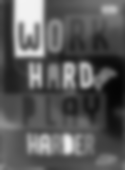
\includegraphics[width=0.05\hsize]{img/o-report-gp-18-0.png}
     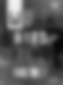
\includegraphics[width=0.025\hsize]{img/o-report-gp-27-0.png}
     \caption{First image of each layer of Gaussian Pyramid}
     \label{fig:gp}
 \end{figure}
 Then, the algorithm look on each layer, and the previous and the next one to look for the most significant gradients on those layers, resulting in a set of candidates for keypoints in a format [x,y,$\sigma$].
 
 After that each is shifted a bit to represent better its position between the layers and to calculate Hessian (used further to discard edges) and it's coordinates are converted to polar. This way, the description collected is about it's surroundings in a radius an direction of it's resultant gradient. The keypoints with low contrast or with a descriptor that looks like an edge instead of corner are discarded using a contrast threshold set to $0.025$.
 
 The Figure~\ref{fig:keypoints} show a comparison between the features detected with OpenCV's SIFT and the SIFT implemented in this work. The foundation of the code was extracted from the following three main sources: the sift paper, the OpenCV explanation\footnote{Introduction to SIFT (Scale-Invariant Feature Transform) \url{<https://opencv-python-tutroals.readthedocs.io/en/latest/py_tutorials/py_feature2d/py_sift_intro/py_sift_intro.html>} accessed on 24/09/2019} and a python tutorial\footnote{Implementing SIFT in Python \url{<https://medium.com/@lerner98/implementing-sift-in-python-36c619df7945>} accessed on 24/09/2019}. The best configuration for SIFT parameter used in the project was: layers of octave = 17, number of octave = 4, sigma = 1.6, and contrast threshold = 0.025.
 
 \begin{figure}
     \centering
     
\includegraphics[width=0.4\hsize]{img/o-kp-0.png}
     
\includegraphics[width=0.4\hsize]{img/o-kp-1.png}
     \caption{Keypoints extracted (colorful circles) on the original template. On the left, the result from the SIFT implemented in this project. On the right, the features extracted using OpenCV's library}
     \label{fig:keypoints}
 \end{figure}


\subsection{Target Frame Detection}

Our video was recorded in an environment with little interference from other objects, so the detection of the keypoint became easier. From this, the target image was provided a priori to the algorithm as an initial artificial frame.

The application of SIFT to this artificial frame resulted in the identification of the keypoints that would later be located in subsequent frames. For this, it was assumed that the target image was at the origin of its coordinate system, so calculating the transformations always mapped the target image to their respective points in the following frames.

The target image was provided in the portrait position, so we knew a priori which points corresponded to the upper and lower corners. The perfect alignment of the source image with the target was achieved by creating a rectangular matrix with the same dimensions as the target image, serving as a mask throughout the process. Thus, it was possible to extract the target image from the frame and perform the addition of the source image, considering the rectangular shape of both.


\subsection{Match Hypothesis}

To find the descriptors between two frames, we use the k-nearest neighbors (KNN) algorithm, this algorithm is widely used in the machine learning community and serves to detect similarities between objects. In this work, KNN was used to detect similarity between descriptors in different frames.

The algorithm takes as parameter two descriptor vectors from SIFT and returns an index vector, also known as matches, which will be used to later retrieve keypoints in the two frames. In our implementation, KNN was used to find 2 clusters, as shown in Listing~\ref{code:least-squares}.


 \begin{lstlisting}[language=Python, caption={K-nearest neighbors}, label={code:knn}]
 def _knn_match(self, query, train, k):
    """
    Perform the match using knn

    Keyword arguments:
    query -- the query vector
    train -- the training vector
    k -- number of clusters
    """

    matches = []

    # For each descriptor in the current
    for i, q in enumerate(query):

        # Get the k-nearest neighbors
        neighbor = self._get_neighbors(train, q, k)

        matches_knn = set()

        # Create the k descriptor tuple
        for n in neighbor:
            matches_knn.add(Match(i, n[0], n[1]))

        matches.append(matches_knn)

    return matches

def _get_neighbors(self, query, train, k):
    """
    Get the k-nearest neighbors

    Keyword arguments:
    query -- the query vector
    train -- the training vector
    k -- number of clusters
    """

    # Create the matrix of distances
    distances = np.zeros((np.shape(query)[0], 2), dtype=np.int)

    # For each pair, calculates the distance
    for x, q in enumerate(query):
        distances[x] = (x, euclidean_distance(train, q))

    # Sort based on distance using numpy notation
    distances = distances[distances[:, 1].argsort()]

    neighbors = []

    # Group in k clusteres
    for x in range(k):
        neighbors.append(distances[x])

    return neighbors
    
\end{lstlisting}

However, to compare points, one should use a distance metric. As we use SIFT to describe the points, the metric used was the distance $L_2$. In this implementation, we performed Hamming distance tests for BRIEF descriptors but chose to follow using SIFT.

The option for 2 clusters was made from the SIFT documentation, where the author, Lowe, uses a threshold of 0.75 between the two clusters to verify the quality of the matches, as shown in Listing~\ref{code:matching}.

\begin{lstlisting}[language=Python, caption={Matching Lowe's Criteria}, label={code:matching}]

def match(self, query, train, k=2):
    """
    Match the query with the train using k-nearest neighbors

    Keyword arguments:
    query -- the query vector
    train -- the training vector
    k -- number of clusters
    """

    matches_knn = self._knn_match(query, train, k)

    # Apply ratio test
    matches = []
    for m, n in matches_knn:
        if m.distance < 0.75*n.distance:
            matches.append(m)

    return matches

\end{lstlisting}

In addition, a class called \textbf{Match()} was implemented to store the similarity between descriptors, as shown in Listing~\ref{code:match}. This class is composed of the indexes of both descriptors and a distance value for them.

\begin{lstlisting}[language=Python, caption={Match Class}, label={code:match}]

class Match:
    """
       A class used to store the match information

       Methods
       -------
       """

    def __init__(self, queryIdx, trainIdx, distance):
        self.queryIdx = queryIdx
        self.trainIdx = trainIdx
        self.distance = distance

\end{lstlisting}

After implementing this code we ran several tests to validate the quality of the results. Below are shown two examples of matches between frames. Figure~\ref{fig:matches_0} shows the matches between the artificial frame and the first frame of the video.

\begin{figure}[H]
     \centering
     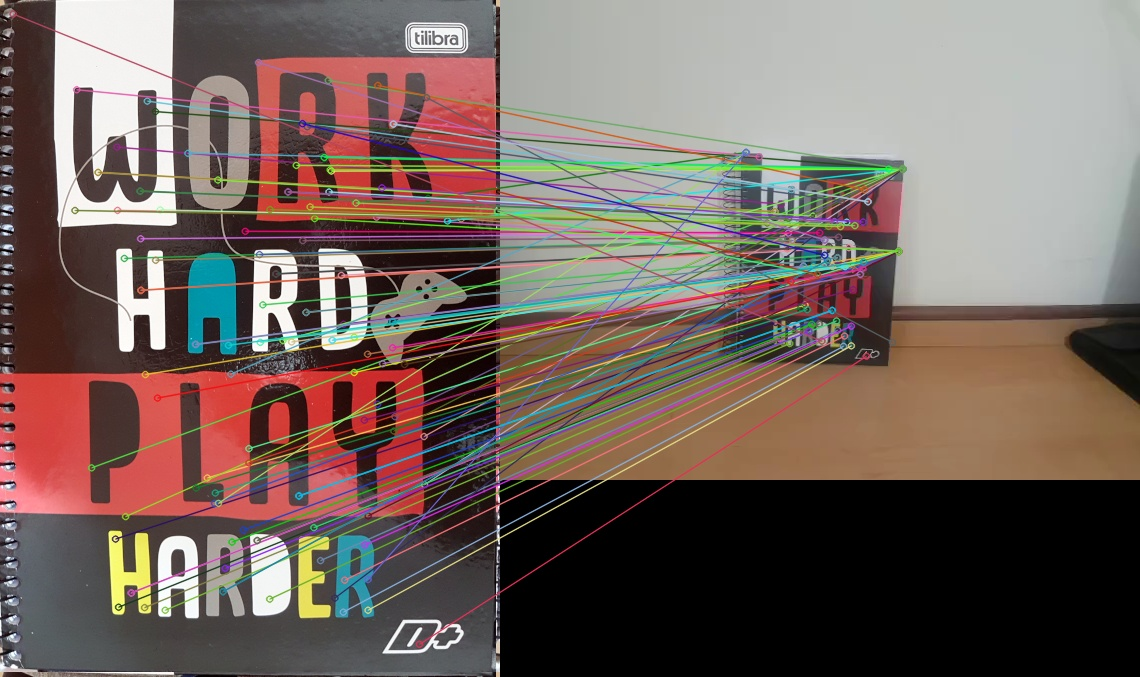
\includegraphics[width=0.9\hsize]{img/matches_0.jpg}
     \caption{Matches between the artifical frame and frame 0.}
     \label{fig:matches_0}
\end{figure}

In Figure~\ref{fig:matches_1} we can see the matches between two frames of the video.

\begin{figure}[H]
     \centering
     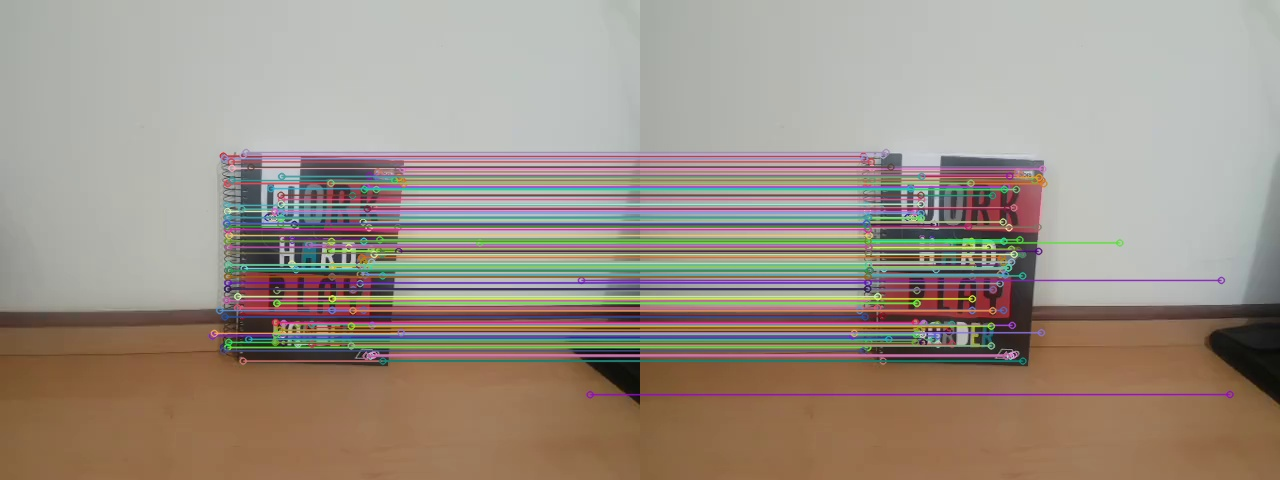
\includegraphics[width=0.9\hsize]{img/matches_1.jpg}
      \caption{Matches between frame 0 and frame 1.}
     \label{fig:matches_1}
\end{figure}

Therefore, the SIFT algorithm was able to detected the same points in both frames and the matching algorithm was able to select them based on their $L_2$ distance. The points are located in regions where the gradient is high, such as the notebook's borders, the letters and regions of high variation in texture. Some points were also located in the wall and in the table, but they were considered outliers.


\subsection{Calculating the Affine Transform between two frames}

To learn the appropriate Affine transform between frames, which is used for estimate the position of the target frame, the candidate keypoint matches from the previous subsection are used here. As the Affine transform has 6 degrees of freedom (associated with rotation and translation in the coordinate system), we need 3 pairs of candidate keypoints in order to find the parameters of the Affine transform matrix such that:

\begin{equation}
    Y = AX
    \label{eq:mat}
\end{equation}

which $Y$ are the candidate match points in the current frame, $A$ is the affine transform matrix and $X$ are the candidate match points in the previous frame. 
Equation \ref{eq:mat} can be explanded for the transformation of one pair of candidate matches as:

\begin{equation}
\begin{bmatrix}
  x_{i}^{'} \\ y_{i}^{'}
\end{bmatrix}  =
\begin{bmatrix}
  a & b & c \\ d & e & f
\end{bmatrix}.
\begin{bmatrix}
  x_{i} \\ y_{i} \\ 1
\end{bmatrix}  
\end{equation}

As we have 6 variables to solve for, we need 3 pairs of candidate matches.

To solve $A$ for three candidate matches, consider equation \ref{eq:mat}. Expanding the equation, we have that:

\begin{equation}
  \begin{bmatrix}
    x_{1} & y_{1} & 1 & 0 & 0 & 0 \\
    0 & 0 & 0 & x_{1} & y_{1} & 1 \\
    x_{2} & y_{2} & 1 & 0 & 0 & 0 \\
    0 & 0 & 0 & x_{2} & y_{2} & 1 \\
    x_{3} & y_{3} & 1 & 0 & 0 & 0 \\
    0 & 0 & 0 & x_{3} & y_{3} & 1 \\
  \end{bmatrix}
  .
  \begin{bmatrix}
      a \\
      b \\
      c \\
      d \\
      e \\
      f
  \end{bmatrix} = 
  \begin{bmatrix}
    x_{1}^{'} \\
    y_{1}^{'} \\
    x_{2}^{'} \\
    y_{2}^{'} \\
    x_{3}^{'} \\
    y_{3}^{'} \\
  \end{bmatrix}
\end{equation}

Using Least Squares for this specific case, we have that A is:

\begin{equation}
  A = (X^{T}X)^{-1}(X^{T}Y)
  \label{eq:ls}
\end{equation}

Listing \ref{code:least-squares} shows our implementation of the Least Squares to solve equation \ref{eq:ls}. As visible, we treat the possibility of $X^{T}.X$ being a singular matrix by returning A as a 0-matrix (bad combination of candidate matches).

 \begin{lstlisting}[language=Python, caption={Least Squares Implementation}, label={code:least-squares}]
  def least_squares(prev_points, curr_points):
    """
    It calculates least squares in order to find affine transform that transforms
    a set of coordinates to another

    Keyword arguments:
    prev_points -- set of original coordinates
    curr_points -- set of transformed coordinates
    """
    n_points = prev_points.shape[0]
    x = np.zeros(shape=(2*n_points, 6), dtype=np.float32)
    for idx, _ in enumerate(prev_points):
        x[2*idx] = [prev_points[idx][0], prev_points[idx][1], 1, 0, 0, 0]
        x[2*idx + 1] = [0, 0, 0, prev_points[idx][0], prev_points[idx][1], 1]

    y = np.zeros(shape=(2*n_points, 1), dtype=np.float32)
    for idx, _ in enumerate(curr_points):
        y[2*idx][0] = curr_points[idx][0]
        y[2*idx + 1][0] = curr_points[idx][1]

    transp_times_x = (np.transpose(x)).dot(x)
    det = np.linalg.det(transp_times_x)

    #Singular Matrix
    if det == 0:
        return np.zeros((6, 1))

    a = (np.linalg.inv(transp_times_x)).dot(((np.transpose(x)).dot(y)))
    return a
\end{lstlisting}

Considering that not necessarily all the candidates are suitable (as mentioned before), we use RANSAC (Random Sample Consensus) to estimate valid candidates for solving the system. This algorithm picks 3 random candidate matches, solves the $A$ matrix using Least Squares and evaluates if $A$ is good by testing it with the candidates themselves. If the calculated $A$ is the best, it holds that $A$. It executes the algorithm $k$ times, removing bad matches from the candidates to be picked to solve $A$ after every good $A$ fit. After $k$ times, it executes Least Squares algorithm one last time to all remaining match candidates to find best possible $A$ for the set, and returns it. Following subsections explain in a more detailed way the full implementation. The RANSAC algorithm explained here is shown in listing \ref{code:ransac}

\begin{lstlisting}[language=Python, caption={RANSAC to estimate Affine Transformation Matrix}, label={code:ransac}]
  def get_affine_transform_matrix(self, previous_f_points, current_f_points):
    """
    It runs RANSAC with least squares to find the affine transform
    matrix for the candidate matches

    Keyword arguments:
    previous_points -- set of original candidate coordinates
    current_points -- set of transformed candidate coordinates
    """
    point_matches = np.zeros((self._n_ransac_iterations, 3, 2), dtype=np.float32)
    best_number_matches = 0
    best_a = []
    previous_f_ransac_set = np.copy(previous_f_points)
    current_f_ransac_set = np.copy(current_f_points)

    # starts RANSAC
    for i in range(self._n_ransac_iterations):
        n_points = len(previous_f_ransac_set)
        # find 3-points combination which was not chosen before
        valid_eq_points = False
        while not valid_eq_points:

            idx = 0
            pf_guess_array = np.full((3, 2), -1)
            cf_guess_array = np.full((3, 2), -1)
            while idx < 3:

                guess = random.randint(0, n_points - 1)
                #if not guess in guess_array:
                if not (pf_guess_array == previous_f_ransac_set[guess]).all(1).any():
                    pf_guess_array[idx][0] = previous_f_ransac_set[guess][0]
                    pf_guess_array[idx][1] = previous_f_ransac_set[guess][1]
                    cf_guess_array[idx][0] = current_f_ransac_set[guess][0]
                    cf_guess_array[idx][1] = current_f_ransac_set[guess][1]
                    idx += 1

            valid_eq_points = not np.any(np.all(pf_guess_array == point_matches, axis=(1, 2)))
        point_matches[i] = pf_guess_array

        # solve least squares for the guess combination
        a = least_squares(pf_guess_array, cf_guess_array)
        n_matches, unmatch_points_idx = self._matches_based_on_affine_matrix(
            previous_f_points, current_f_points, a)

        # if the number of matches obtained this time is greater than previous iterations, 
        # we have a new best affine transform matrix
        if n_matches > best_number_matches:
            best_number_matches = n_matches
            best_a = a
            match_rate = best_number_matches/len(previous_f_points)
            # if it achieves considerably good success rate, we can remove outlier candidates
            if match_rate > self._success_rate/2:
                idx_to_be_deleted = []
                for idx in unmatch_points_idx:
                    m = (previous_f_ransac_set == previous_f_points[idx]).all(1)
                    idx = np.where(m == True)
                    for el in idx[0]:
                        idx_to_be_deleted.append(el)
                previous_f_ransac_set = np.delete(
                    previous_f_ransac_set, idx_to_be_deleted, axis=0)
                current_f_ransac_set = np.delete(
                    current_f_ransac_set, idx_to_be_deleted, axis=0)

    # solve least squares one last time with all the survivor candidates
    a_final = least_squares(previous_f_ransac_set, current_f_ransac_set)
    n_matches, unmatch_points_idx = self._matches_based_on_affine_matrix(
        previous_f_points, current_f_points, a_final)
    if n_matches > best_number_matches:
        best_a = a_final
        best_number_matches = n_matches

    return np.reshape(best_a, (2, 3))
\end{lstlisting}

\subsubsection{Number of RANSAC Iterations}
  As RANSAC is a stochastic algorithm, we need to estimate the minimum number of executions to have selected at least 1 group of three candidate match points that can solve the system and have a good A. It depends on probability functions, such as the probability good of inliers in our set (probability of good candidates in our system) and the success rate (how good the final matrix A has to be to solve the system). 

  The number of iterations can be estimated, as descibed in the literature, as

  \begin{equation}
    k = \dfrac{\log (1 - P_{success})}{\log (1 - (P_{inliers})^{2})}
  \end{equation}

  Listing \ref{code:k} shows the function to calculate the number of iterations. We use the ceiling of the result of the division.

  \begin{lstlisting}[language=Python, caption={Calculate number of RANSAC iterations}, label={code:k}]
    def _calculate_ransac_iterations(self):
      """
      It calculates the number of ransac iterations needed based
      on the probability of inliers in set and the desired success rate
      """
      n = math.log(1 - self._success_rate)/math.log(1 - (self._inliers_rate)**2)
      self._n_ransac_iterations = int(math.ceil(n))
  \end{lstlisting}

\subsubsection{Evaluate calculated Affine Transform Matrix}
In order to evaluate the calculated Affine Transform matrix, equation \ref{eq:mat} is solved for the $X$ candidate points from the previous frame and the $A$ matrix, and then the $Y$ points are evaluated using the candidate points from the current frame using the distance between each of them. These distances are then normalized and the ones smaller than a threshold are considered correct matches. The number of matches and the indexes of not matched points are returned to the main RANSAC algorithm. Listing \ref{code:eval} shows the implementation of the method. 

\begin{lstlisting}[language=Python, caption={Evaluates calculated Affine Transform matrix}, label={code:eval}]
  def _matches_based_on_affine_matrix(self, previous_points, current_points, a):
    """
    It measures how good is the calculate affine transform matrix
    based on the threshold and candidate matches

    Keyword arguments:
    previous_points -- set of original coordinates
    current_points -- set of transformed coordinates
    """
    n_match_points = 0
    unmatch_points_idx = []
    distances = []

    for idx, point in enumerate(previous_points):
        tf_x = a[0][0]*point[0] + a[1][0]*point[1] + a[2][0]
        tf_y = a[3][0]*point[0] + a[4][0]*point[1] + a[5][0]
        distance = points_distance(current_points[idx][0], tf_x, current_points[idx][1], tf_y)
        distances.append(distance)

    max_d = np.max(distances)

    normalized_distance = []
    for d in distances:
        normalized_distance.append(d/max_d)

    for idx, n_d in enumerate(normalized_distance):
        if n_d < self._threshold:
            n_match_points += 1
        else:
            unmatch_points_idx.append(idx)

    return n_match_points, unmatch_points_idx
\end{lstlisting}


\subsection{Video Augmentation}

The video augmentation was performed by applying the affine matrix to each pixel of the source image. So that each pixel was mapped to their respective coordinates in the frame image. For this, the \textbf{warpAffine} method has been implemented as shown in Listing~\ref{code:warpAffine}.

\begin{lstlisting}[language=Python, caption={Warp Affine Method}, label={code:warpAffine}]
def _warpAffine(self, source, a_matrix, shape):
    
    # Define the new shape
    new_shape = (shape[0], shape[1], 3)
    
    # Create the empty new image
    new_image = np.zeros(new_shape, dtype=np.uint8)
    
    # Separate the rotation matrix
    a = a_matrix[:,0:2]
    
    # Separate the translation matrix
    b = a_matrix[:,2:3]
    
    # Convert to homogeneous coordinates
    a = np.hstack((np.flip(a), np.flip(b)))
    a = np.vstack((a, [0,0,1]))
    
    for y in range(source.shape[0]):
        for x in range(source.shape[1]):
            
            # Build the point
            p = np.array([y, x, 1])

            # Apply the affine transformation
            y_1, x_1, _ = np.matmul(a, p)
            
            if y_1 < 0:
                y_1 = 0
                
            if x_1 < 0:
                x_1 = 0
            
            if y_1 >= shape[0]:
                y_1 = shape[0]-1
                
            if x_1 >= shape[1]:
                x_1 = shape[1]-1
            
            new_image[int(y_1), int(x_1), :] = source[y, x, :]
    
    return new_image

\end{lstlisting}

This method receives an image that will be modified, a affine matrix in homogeneous coordinates and a dimension for the resulting image. The result of applying this method in our project is shown in Figure~\ref{fig:paste_0}.

\begin{figure}[H]
     \centering
     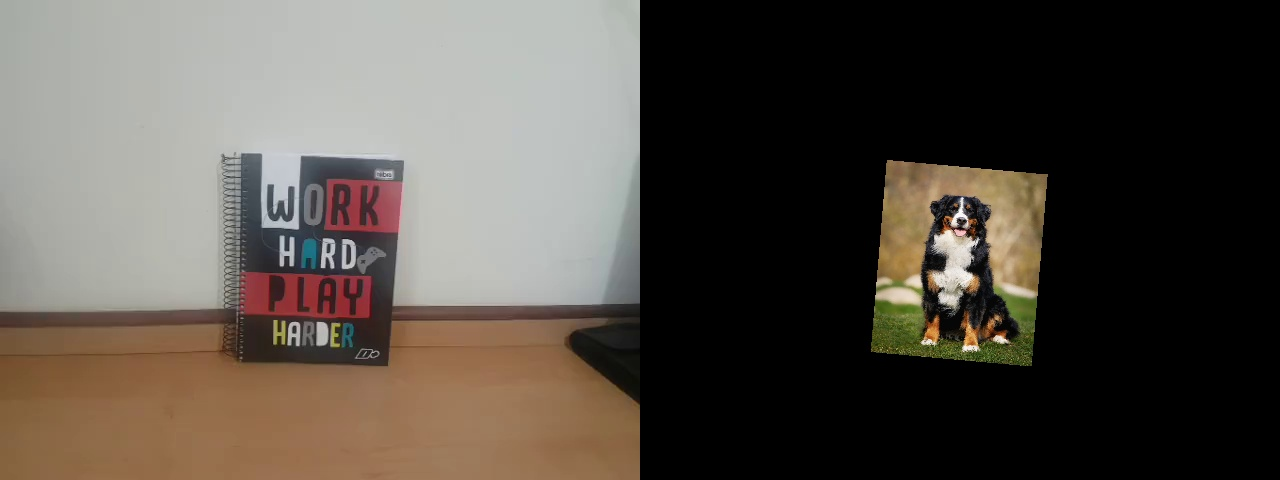
\includegraphics[width=0.9\hsize]{img/paste_0.jpg}
     \caption{Warp the source image with the same frame size as the target one.}
     \label{fig:paste_0}
\end{figure}

The resulting image has the same dimensions as the video frame, making augmentation simpler as you simply apply a mask to both images to crop the backgound and foreground. In this case, we do not need to resize the source image, once we considered that same dimension as the frame, so the source image could be mapped exactly to the target position. The procedure for accomplishing this task is shown in Listing~\ref{code:augmentation}.

\begin{lstlisting}[language=Python, caption={Augmentation algorithm}, label={code:augmentation}]
# Warp the source image
source = self._warpAffine(self.source, a_all, (current_frame.shape[0], current_frame.shape[1]))

# Warp the mask
target_mask = self._warpAffine(self.initial_target_mask, a_all, (current_frame.shape[0], current_frame.shape[1]))

# Convert it to gray scale
target_mask_gray = cv2.cvtColor(target_mask, cv2.COLOR_BGR2GRAY)

# Define the threshold to separate foreground from background
_, mask = cv2.threshold(target_mask_gray, 150, 255, cv2.THRESH_BINARY_INV)

# Get the inverted mask
mask_inv = cv2.bitwise_not(mask)

# Get the background image
background = cv2.bitwise_and(current_frame, current_frame, mask=mask)

# Get the foreground image
foregound = cv2.bitwise_and(source, source, mask=mask_inv)

# Add both images
output_frame = cv2.add(background, foregound)
\end{lstlisting}


The result after applying this procedure is the creation of a mask with the same dimensions as the target image that we want to crop from the frame. To perform this step it is necessary to assume that the mask has the same dimensions as the source image, that is, the affine transformations are also performed on the mask. This allows us to apply a threshold value and identify exactly where the mask should be. After that, we just apply a binary operator AND to define the foreground and background portions of the images, as shown in Figure~\ref{fig:paste_1}.

\begin{figure}[H]
     \centering
     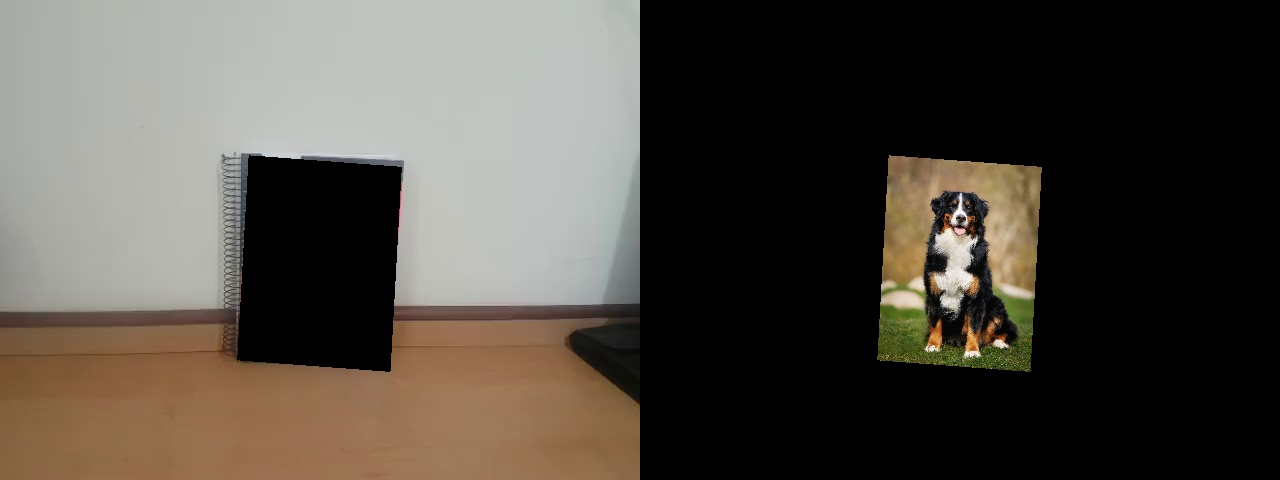
\includegraphics[width=0.9\hsize]{img/paste_1.jpg}
      \caption{Extract the background using a mask.}
     \label{fig:paste_1}
\end{figure}

After extracting background and foreground portions, we just add the source transformed image with the frame without the target image. After that, we repeat the whole process for each frame.

\section{Experiments and Discussion}

The \textbf{main.py} file executes our test pipeline. The idea is the following: for the input video (\textbf{input/i-0.mp4}), a target object in every frame of the input (\textbf{{input/i-2.jpg}}) is substituted by another image (\textbf{input/i-1.jpg}). To test two different strategies for mapping the target in the video, two execution stages are created: in one stage, the target is tracked comparing a pair of video frames ($frame_{i - 1}$ and $frame_{i}$), for every consecutive pair of frames (using the artificial frame for the first one). In the other stage, the frame ($frame_{i}$) is compared with the target. Figure \ref{fig:target-and-image} shows the input images. The results of each approach is listed in the following subsections.
The input video has the following characteristics: starting the target in the central region of the video, perform camera translations from left to right, perform a zoom-out, top-down translations, clock-wise rotation (full path), zoom-in, counterclock-wise rotation. The duration of the video is approximately 20 seconds.

\begin{figure}[H]
  \centering
  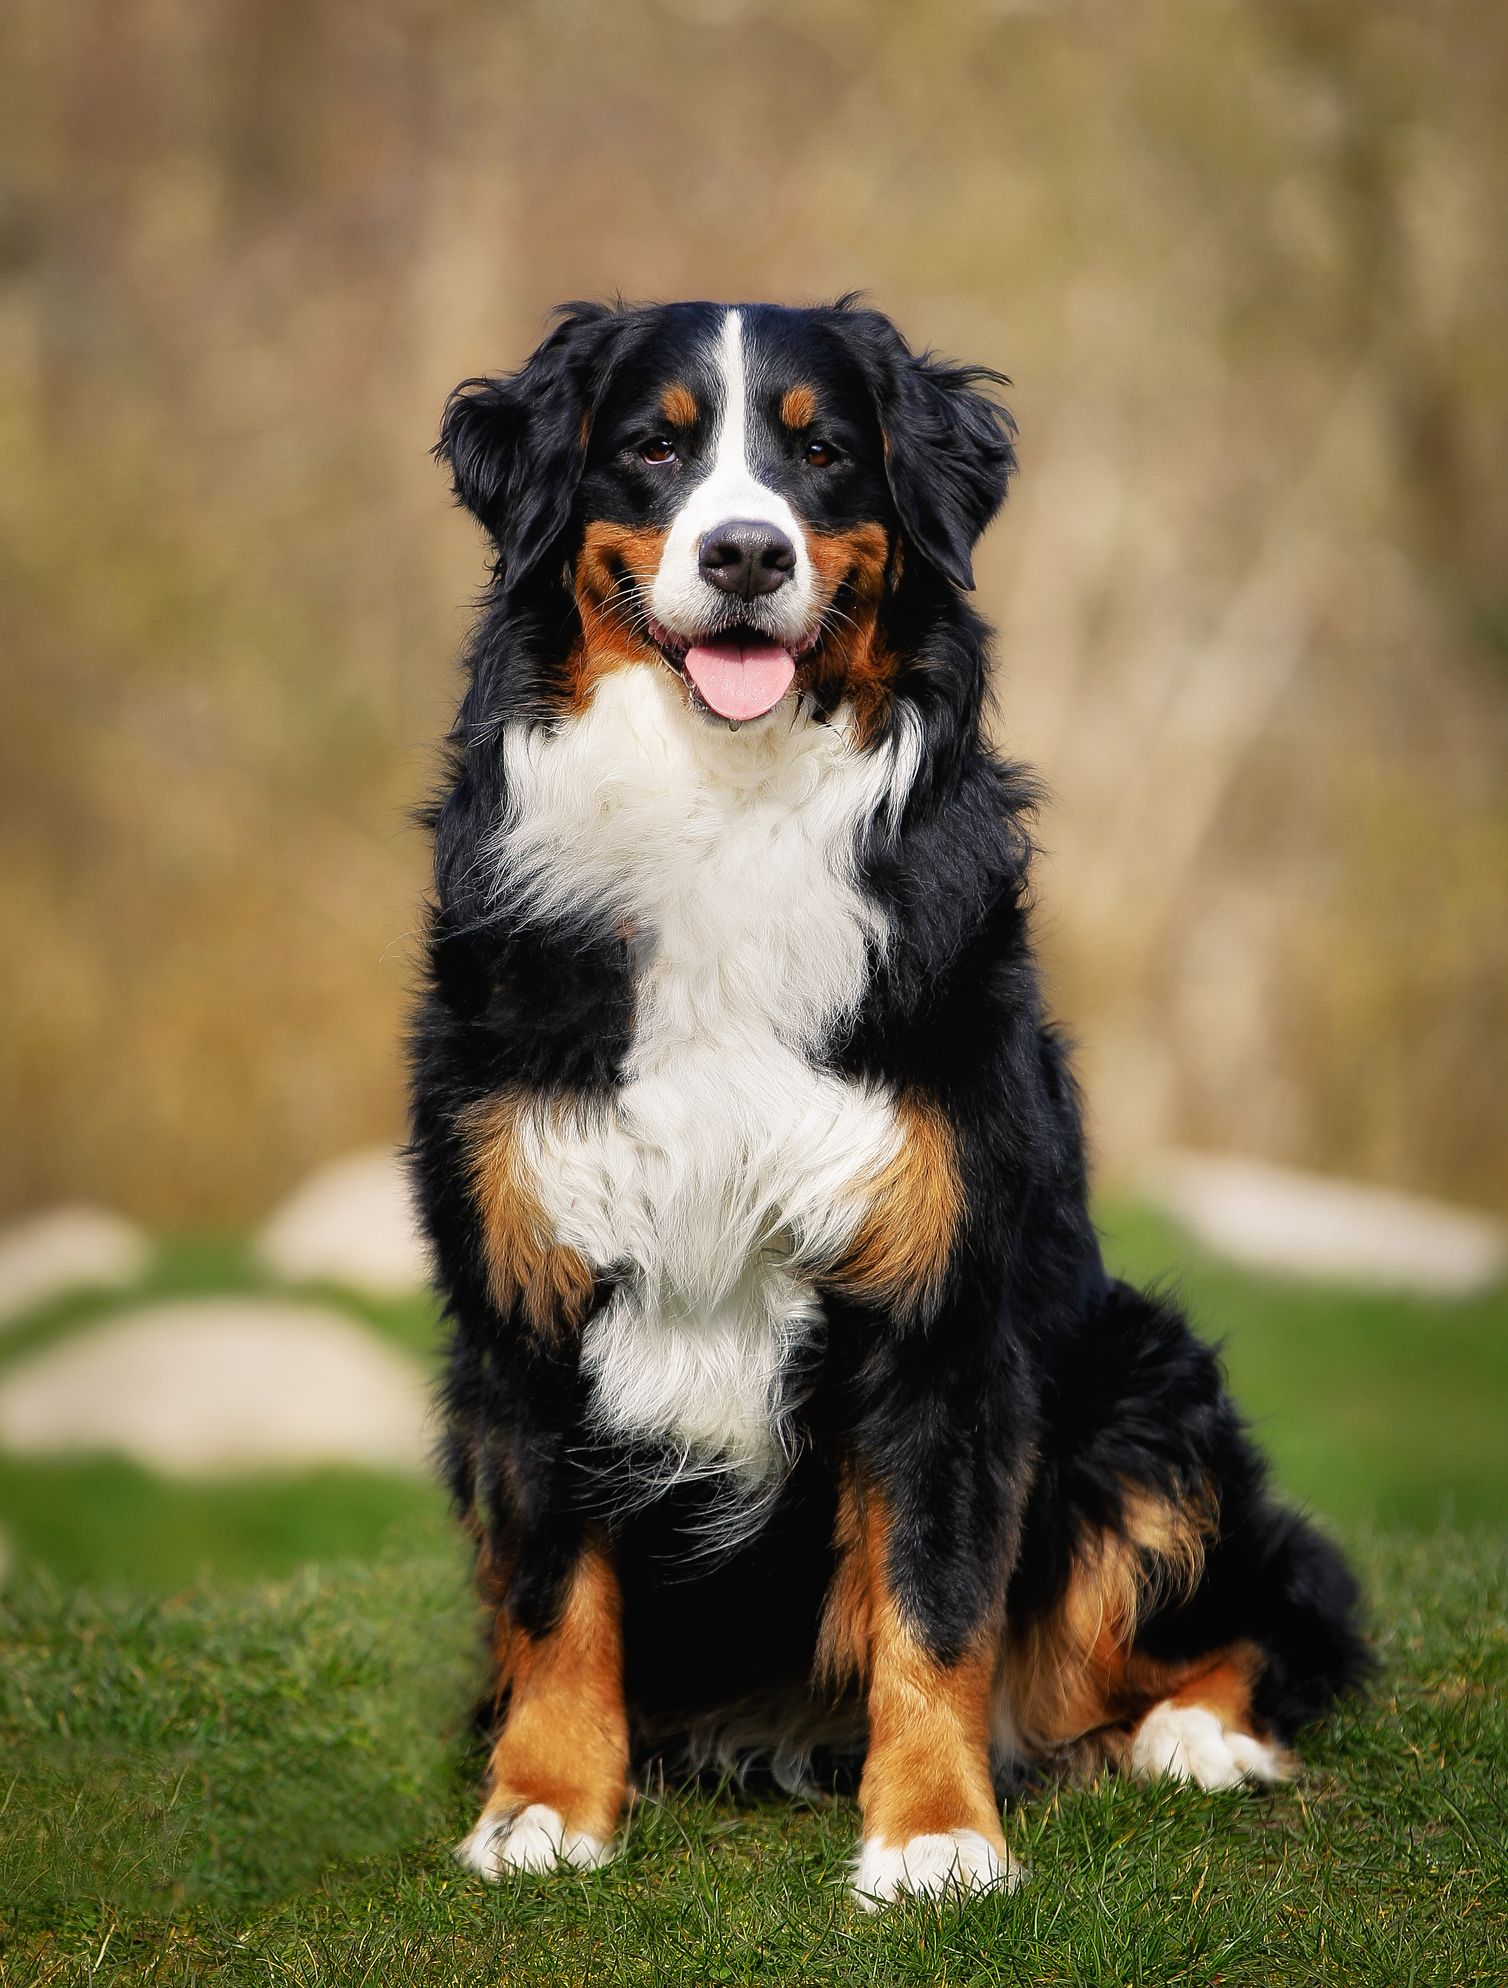
\includegraphics[width=0.4\hsize]{../input/i-1.jpg}
  
\includegraphics[width=0.4\hsize]{../input/i-2.jpg}
  \caption{Input images for AR solution. a) Image to be pasted in every frame b) Target Frame to be substituted in every frame.}
  \label{fig:target-and-image}
\end{figure}

\subsection{Tracking the Target between video frames}

The first test performed was to execute the video augmentation using the frame-by-frame criteria to calculate the affine transformation. As we can see from Figure~\ref{fig:frame-by-frame}, the quality of the image paste gets worse as the frames are sequentially changed.

\begin{figure}[H]
  \centering
  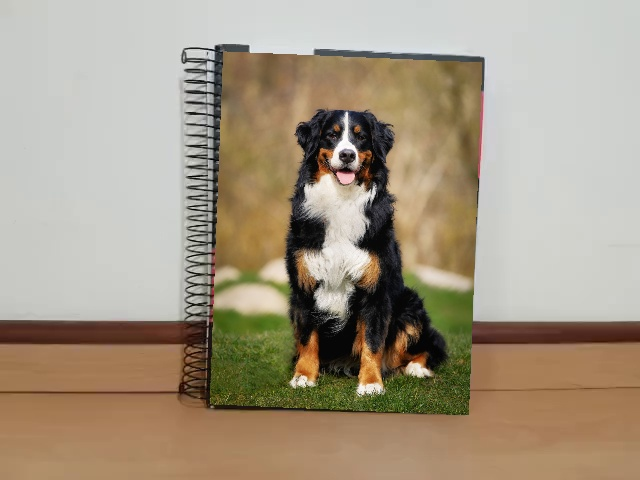
\includegraphics[width=0.31\hsize]{img/frame-by-frame_0.jpg}
  
\includegraphics[width=0.31\hsize]{img/frame-by-frame_1.jpg}
  
\includegraphics[width=0.31\hsize]{img/frame-by-frame_2.jpg}
  \caption{Augmented images compared frame-by-frame.}
  \label{fig:frame-by-frame}
\end{figure}

 The paste area gets descentralized from the target frame, and the pasted image distorted.
Considering the fact that we are using the Affine Transform to track the target frame from one video frame to the other, we have accumulated error during execution, as, for example, the Affine transform of frame $i + 2$ depends on the Affine Transform of frame $i$ to $i + 1$ and the one of frame $i + 1$ to $i + 2$, and each Affine Transform has an associated error within its calculation (number of RANSAC iterations, incapability of removing bad matching candidates, inconsistencies on calculated keypoints). Also, as we use an Affine Transform, it deals with limited number of degrees of freedom, considering the camera movement and frame distortion (the recorded video might insert camera movements that could only be correctly estimated in using a projection transform).

\subsection{Tracking the Target comparing to the Artificial Frame}

In order to decrease the error across all the frames, we perform this test comparing the frame with its artificial one. From Figure~\ref{fig:frame-by-source}, comparing to the previous case, we can see an improvement of the pasting result.

\begin{figure}[H]
  \centering
  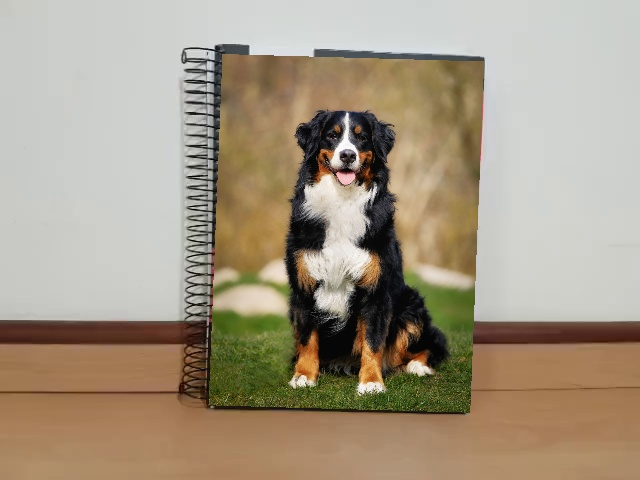
\includegraphics[width=0.31\hsize]{img/frame-source_0.jpg}
  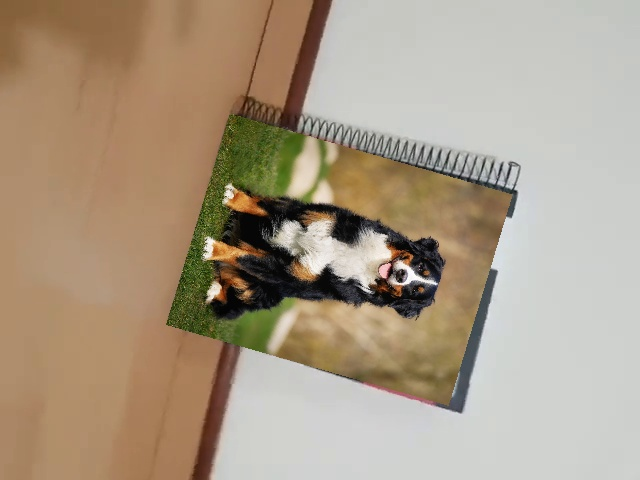
\includegraphics[width=0.31\hsize]{img/frame-source_1.jpg}
  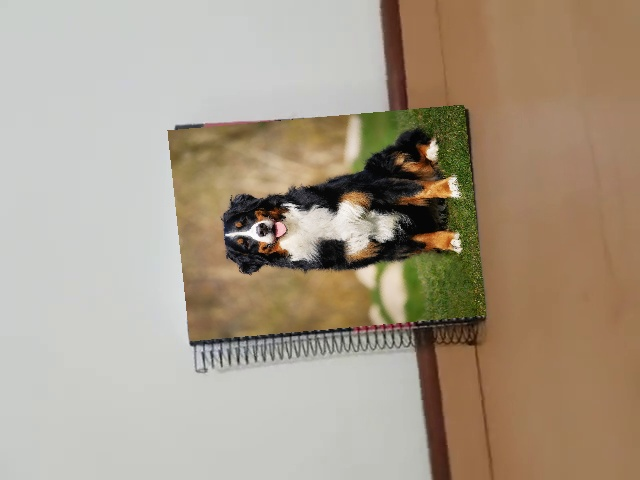
\includegraphics[width=0.31\hsize]{img/frame-source_2.jpg}
  \caption{Augmented images compared frame-by-source.}
  \label{fig:frame-by-source}
\end{figure}

As we do not have error accumulation from one frame to the other, the transform deals better with the target movement. It is still present some error due to degree of freedom limitation of the Affine Transform. 

\section{Contribution Matrix}

The contribution of each author is presented below.

\begin{table}[H]
\begin{tabular}{|l|l|}
\hline
\textbf{Task}                       & \textbf{Author} \\ \hline
SIFT Implementation                 & Leonardo      \\ \hline
Target Frame and Video Augmentation & Iury          \\ \hline
Matching Algorithm                  & Iury          \\ \hline
Affine Transformation               & Thales        \\ \hline
RANSAC and Least Squares            & Thales        \\ \hline
\end{tabular}
\end{table}

\section{Conclusion}

In this work, an augmented reality algorithm was implemented to insert an image into a specific portion of a video. For this, a feature detection and description algorithms were developed, we chose to use SIFT because it has a lot of material available, also, this algorithm provides a higher detection quality than the others.

In addition, a matching algorithm was implemented. In this work, k-nearest neighbors were implemented using two clusters. After the matches were found, the affine transformations matrix was found, using RANSAC, both algorithms were implemented, as well as the calculation of iterations. For matrix estimation, the least-squares algorithm was also implemented.

After that, the affine matrix was applied to the pixels of the source image, to transform it into the frame space. In the sequence, video augmentation was performed using a mask to separate the frame's background and foreground. After this step, the insertion of the desired image in place of the target image was performed simply by summing the image with the frame.

With the code implemented, two tests were performed to reduce the accumulated error. Frame-by-frame comparison generates a lot of errors in the affine matrix, due to a poor keypoint detection during the execution of the algorithm. One way to solve this has been found by comparing it to the artificial frame, so the error is never carried forward.

Finally, the execution of this work gave us a better understanding of how the affine matrix detection, matching, and generation algorithms work internally.

\end{document}
